% Rapport d'avancement Dream in Orbit. Compilation : tectonic rapport.tex (ou xelatex).
% Les figures viennent de figures.py (voir l'annexe).
\documentclass[11pt,a4paper]{article}

\usepackage{fontspec}
\usepackage{unicode-math}
\setmainfont{texgyreschola}[Extension=.otf, UprightFont=*-regular, BoldFont=*-bold,
  ItalicFont=*-italic, BoldItalicFont=*-bolditalic]
\setmathfont{texgyreschola-math.otf}
\setmonofont{texgyrecursor}[Extension=.otf, UprightFont=*-regular, BoldFont=*-bold, Scale=0.9]
\usepackage{polyglossia}
\setmainlanguage{french}

\usepackage[a4paper,margin=2.3cm,top=2.2cm,bottom=2.4cm]{geometry}
\usepackage{microtype}
\usepackage{graphicx}
\usepackage{booktabs}
\usepackage{tabularx}
\usepackage{array}
\usepackage[table]{xcolor}
\usepackage{caption}
\usepackage{float}
\usepackage{enumitem}
\usepackage{tikz}
\usetikzlibrary{positioning,arrows.meta,fit,calc}
\usepackage{fancyhdr}
\usepackage[hidelinks]{hyperref}

\definecolor{bleu}{HTML}{2A78D6}
\definecolor{orange}{HTML}{EB6834}
\definecolor{encre2}{HTML}{52514E}
\definecolor{fond}{HTML}{F3F2EE}
\definecolor{trait}{HTML}{9A9890}

\captionsetup{font=small,labelfont=bf,labelsep=period,justification=justified,singlelinecheck=false}
\setlist{itemsep=2pt,topsep=4pt}
\setlength{\parskip}{4pt}
\renewcommand{\arraystretch}{1.12}
\newcommand{\code}[1]{\texttt{#1}}
\setlength{\emergencystretch}{2em}
\newcolumntype{R}{>{\raggedleft\arraybackslash}X}

\pagestyle{fancy}
\fancyhf{}
\fancyhead[L]{\small\color{encre2}Dream in Orbit, rapport d'avancement}
\fancyhead[R]{\small\color{encre2}4 novembre 2026}
\fancyfoot[C]{\small\color{encre2}\thepage}
\renewcommand{\headrulewidth}{0.4pt}

\begin{document}

\thispagestyle{plain}
\begin{center}
  {\LARGE\bfseries Dream in Orbit}\\[4pt]
  {\large Rapport d'avancement : world model de la consommation électrique d'un satellite}\\[8pt]
  {\color{encre2}Max DENIS \quad·\quad 4 novembre 2026 \quad·\quad branche \code{ameliorations}, commit \code{79f10c1}}
\end{center}

\vspace{4pt}
\noindent\colorbox{fond}{\parbox{\dimexpr\linewidth-2\fboxsep}{\small
\textbf{État au 4 novembre.} Le modèle final est un ensemble de 10 world models GRU (deux jeux de variables, cinq graines chacun). Il obtient une RMSE de 0.0853 en validation directe (entraînement sur annee1, simulation de annee2) et de 0.0940 en validation inverse, soit 0.0897 en moyenne. La prédiction constante fait 0.1155 et le meilleur modèle classique (gradient boosting) 0.0975. Le dépôt contient \code{train.py}, \code{predict.py} conforme à l'interface, les poids (6.9 Mo), les ablations et la figure « rêve contre réalité ». Le bonus pilote n'est pas commencé et la durée d'entraînement sur GPU T4 n'a pas été mesurée.}}

\vspace{6pt}
Ce rapport suit l'ordre du travail. Les sections 1 à 3 décrivent les données, le protocole de validation et les méthodes essayées avant la solution actuelle, avec ce que chaque essai a appris. Les sections 4 et 5 présentent la solution actuelle et ses résultats : architecture, entraînement, dérive sur la période simulée, erreurs par circuit, incertitude et ablations. Tous les scores sont des RMSE calculées par \code{evaluate.py} ; ils sont écrits avec un point décimal, comme dans la sortie du script.

%=====================================================================
\section{Les données}

Le kit contient deux périodes consécutives de télémétrie réelle. annee1 va du 22/08/2008 au 09/07/2010 et annee2 du 10/07/2010 au 26/05/2012. Chaque période dure 687 jours, soit 16\,488 heures : les noms « annee1 » et « annee2 » ne désignent pas des années civiles. Les deux périodes se suivent à une heure près.

\begin{table}[!htb]
\centering\small
\caption{Fichiers du kit et nombre de lignes par période (comptes de la première exploration des données).}
\label{tab:fichiers}
\begin{tabularx}{\linewidth}{l X r r}
\toprule
Fichier & Contenu d'une ligne & annee1 & annee2 \\
\midrule
\code{power.csv}  & courant mesuré sur les 33 circuits (une mesure toutes les 32 s environ) & 1\,830\,121 & 1\,768\,248 \\
\code{dmop.csv}   & commande envoyée à un sous-système & 187\,126 & 143\,802 \\
\code{ftl.csv}    & intervalle de pointage, avec ou sans communication & 19\,571 & 20\,051 \\
\code{saaf.csv}   & angles du Soleil par rapport au satellite & 1\,261\,290 & 1\,305\,759 \\
\code{evtf.csv}   & événement daté (éclipse, occultation, péricentre\ldots) & 76\,776 & 75\,208 \\
\code{ltdata.csv} & valeurs journalières (distances Soleil et Terre, durée des éclipses) & 687 & 687 \\
\bottomrule
\end{tabularx}
\end{table}

La cible est la moyenne horaire de chaque circuit. Une heure sans mesure reste inconnue et n'est pas notée : 32 heures sont vides dans annee1 et 246 dans annee2 (le plus long trou dure 23 heures). Trois constats de l'exploration ont orienté la suite.

Les circuits ont des amplitudes très différentes. NPWD2451 et NPWD2551 ont des écarts-types de 0.84 et 0.61 sur annee1, alors que NPWD2691 reste presque constant. La RMSE agrège toutes les cellules (heure, circuit) sans pondération, donc les circuits les plus variables pèsent le plus dans le score.

Le niveau moyen de certains circuits change d'une période à l'autre (tableau~\ref{tab:niveaux}). Un modèle qui apprend le niveau d'annee1 se trompe d'office sur ces circuits en annee2. Ce problème est revenu à chaque étape du projet.

Les fichiers de contexte ont des cadences différentes et des recouvrements. \code{ftl} contient 695 intervalles qui chevauchent le précédent dans annee1 ; \code{dmop} s'arrête 12.6 jours avant la fin de \code{power} dans annee2. Il faut donc tout ramener sur une grille horaire commune sans additionner deux fois les durées.

\begin{table}[!htb]
\centering\small
\caption{Les quatre plus grands changements de niveau moyen entre les deux périodes (mesures brutes).}
\label{tab:niveaux}
\begin{tabular}{l r r r}
\toprule
Circuit & Moyenne annee1 & Moyenne annee2 & Écart \\
\midrule
NPWD2851 & 0.201 & 0.323 & $+0.122$ \\
NPWD2531 & 0.119 & 0.011 & $-0.108$ \\
NPWD2532 & 1.232 & 1.319 & $+0.087$ \\
NPWD2451 & 0.645 & 0.685 & $+0.040$ \\
\bottomrule
\end{tabular}
\end{table}

%=====================================================================
\section{Protocole de validation}

\code{make\_validation.py} transforme une période en dossier de test au format de l'évaluation : contextes complets, 7 premiers jours de courants (\code{power\_init.csv}) et liste des heures à prédire. J'ai utilisé deux directions :
\begin{itemize}
  \item directe : entraînement sur annee1, simulation de annee2 (dossier \code{validation/}) ;
  \item inverse : entraînement sur annee2, simulation de annee1\\
  (dossier \code{validation\_inverse/}).
\end{itemize}
Le score de référence est la moyenne des deux RMSE. La seconde direction écarte les réglages qui ne marchent que dans un sens ; le recalage constant du boosting (section~3.2) en est un exemple. Chaque essai passe par la chaîne complète \code{train.py}, \code{predict.py}, \code{evaluate.py} (script \code{outils/valider.py}), jamais par un découpage aléatoire des heures.

Un changement n'est gardé que s'il fait baisser la moyenne. J'ai mesuré le bruit dû à la graine aléatoire sur le premier world model : environ 0.0015 sur la moyenne. Pendant la dernière session, la règle est devenue plus stricte : gain d'au moins 0.0015 sans dégrader aucune direction, ou confirmation sur une seconde série de graines (5 à 9) quand le gain est compris entre 0.0005 et 0.0015.

%=====================================================================
\section{Méthodes essayées avant la solution actuelle}

\subsection{Préparation horaire des contextes}

\code{dio/prepare.py} transforme les cinq fichiers de contexte en 65 variables horaires. Le schéma (codes retenus, valeurs de remplissage) est appris sur annee1 puis réutilisé tel quel sur toute autre période. Aucun courant, même initial, n'entre dans ces variables.

\begin{table}[!htb]
\centering\small
\caption{Les 65 variables horaires produites par \code{dio/prepare.py}.}
\label{tab:variables}
\begin{tabularx}{\linewidth}{l r X}
\toprule
Source & Nombre & Contenu \\
\midrule
\code{ftl}    & 18 & minutes passées dans chacun des 14 modes de pointage, minutes de communication, de couverture et de chevauchement \\
\code{dmop}   & 15 & nombre de commandes pour les 10 codes les plus fréquents, autres codes, total, heures depuis la dernière commande, indicateurs de bord \\
\code{evtf}   & 15 & minutes d'ombre, de pénombre et d'occultation, passages au péricentre et à l'apocentre, comptes d'événements \\
\code{saaf}   & 10 & moyenne et étendue horaires des quatre angles solaires, couverture des mesures \\
\code{ltdata} & 7  & distances Soleil--Mars et Terre--Mars, constante solaire, durées d'éclipse et d'occultation \\
\bottomrule
\end{tabularx}
\end{table}

\subsection{Baselines : constante, Ridge, gradient boosting}

La prédiction constante (moyenne de chaque circuit sur la période d'entraînement) donne 0.1058 en directe et 0.1252 en inverse. Une régression Ridge heure par heure sur les 65 variables descend à 0.0994 en directe.

Le diagnostic de la Ridge sur NPWD2531 montre bien le problème des niveaux. Sur annee1, ce circuit suit la distance au Soleil avec une corrélation de $-0.998$. La Ridge apprend cette relation et l'extrapole sur annee2, où le circuit est presque éteint (moyenne 0.014 au lieu de 0.125). Sa RMSE sur ce circuit monte à 0.208, contre 0.138 pour une simple constante. Une relation très nette sur une période peut donc être fausse sur la suivante.

J'ai ensuite entraîné un gradient boosting par circuit (\code{HistGradientBoostingRegressor}), sans mémoire, puis ajouté un recalage : on décale chaque circuit d'une fraction de l'écart observé sur les 7 jours de \code{power\_init}. Le tableau~\ref{tab:boosting} résume les essais.

\begin{table}[!htb]
\centering\small
\caption{Essais de gradient boosting. Les modèles les plus simples généralisent le mieux d'une période à l'autre.}
\label{tab:boosting}
\begin{tabularx}{\linewidth}{X r r r}
\toprule
Réglage & Directe & Inverse & Moyenne \\
\midrule
300 itérations, 31 feuilles, sans recalage & 0.0981 & 0.1095 & 0.1038 \\
+ recalage constant, poids 0.25 & 0.0970 & 0.1073 & 0.1021 \\
+ recalage qui s'estompe (poids 1, demi-vie 1440 h) & 0.0974 & 0.1020 & 0.0997 \\
600 itérations, 63 feuilles & 0.0994 & 0.1041 & 0.1018 \\
150 itérations, 15 feuilles, au moins 200 observations par feuille & 0.0959 & 0.0994 & 0.0977 \\
\rowcolor{fond} \textbf{100 itérations, 7 feuilles, au moins 500 obs. par feuille + recalage (retenu)} & \textbf{0.0951} & \textbf{0.0999} & \textbf{0.0975} \\
\bottomrule
\end{tabularx}
\end{table}

Deux enseignements sont passés dans le world model. Un recalage constant sur toute la période dégrade l'inverse (0.139 avec un poids de 1) : le niveau des 7 premiers jours n'est fiable que quelques semaines, il faut donc qu'il s'estompe. Et plus le modèle est contraint, mieux il passe d'une période à l'autre, ce qui laisse prévoir que le réseau devra être fortement régularisé.

\subsection{Premier world model GRU et diagnostic de son échec}

Le premier GRU, entraîné sur des fenêtres de 7 jours de démarrage et 60 jours de simulation, faisait 0.1148 en directe, plus mal que le boosting. Le passage à des épisodes d'un an coupés en morceaux de 30 jours (rétropropagation tronquée, l'état caché passant d'un morceau au suivant) l'a amené à 0.1094. Les essais suivants (60 ou 150 pas, sans \code{ltdata}, réseau plus petit et plus de dropout) restaient entre 0.107 et 0.133.

L'erreur augmentait au fil de la période simulée : 0.075 sur les premières semaines, 0.14 à 0.17 en fin de période. Pour savoir si la récurrence était en cause, j'ai entraîné un MLP sans aucune mémoire : il faisait pire (0.156), donc le problème venait des entrées. Plus précisément, 17 variables presque constantes sur annee1 (\code{saaf\_coverage\_fraction}, \code{saaf\_missing}, les indicateurs \code{*\_unknown} et \code{*\_outside\_recorded\_range}) avaient un écart-type minuscule. Dès qu'elles bougent sur annee2 (la couverture \code{saaf} change sur 61 \% des heures), leurs valeurs centrées-réduites deviennent énormes et le réseau sort de son domaine.

La correction tient en trois règles. Une variable dont la valeur la plus fréquente couvre au moins 99.5 \% des heures d'entraînement est écartée. Chaque variable est bornée à sa plage d'entraînement. Les valeurs centrées-réduites sont bornées à $\pm 5$. Avec 48 variables sur 65, le GRU passe à 0.0901 en directe et 0.0989 en inverse, et devient meilleur que le boosting dans les deux directions.

\subsection{Variables supplémentaires, ensembles et itérations}

Avec une seule trajectoire d'environ deux ans pour apprendre, ajouter des variables fait vite surapprendre. La version v2 complète (399 variables : moyennes glissantes passées et futures sur 3, 6, 12 et 24 heures, temps depuis le dernier et jusqu'au prochain événement, phase orbitale, cosinus et sinus des angles) dégrade la moyenne à 0.1025. L'état « dernière commande » des 12 sous-systèmes \code{dmop} corrèle à 0.75 avec NPWD2551 sur annee1, mais fait 0.0973 en directe : la relation est propre à une période. Seule une version réduite, v2r, limitée aux éclipses, aux communications, à la phase orbitale et aux angles, reste au niveau de v1.

Les essais suivants sont listés dans le tableau~\ref{tab:iterations}. Les gains retenus viennent de l'ensemble de graines, du bruit sur les entrées et du mélange de deux jeux de variables. La figure~\ref{fig:progression} reprend la progression complète.

\begin{table}[!htb]
\centering\small
\caption{World models GRU : essais successifs. Les lignes grisées sont les configurations retenues à chaque étape.}
\label{tab:iterations}
\begin{tabularx}{\linewidth}{X r r r}
\toprule
Essai & Directe & Inverse & Moyenne \\
\midrule
\rowcolor{fond} GRU v1, 1 graine, variables filtrées (E2) & 0.0901 & 0.0989 & 0.0945 \\
Variables v2 complètes, 399 variables & 0.0990 & 0.1061 & 0.1025 \\
v1 + état des sous-systèmes \code{dmop} & 0.0973 & -- & -- \\
v2r, 1 graine & 0.0878 & 0.0987 & 0.0933 \\
\rowcolor{fond} Ensemble de 5 graines, v1 (E3) & 0.0876 & 0.0975 & 0.0925 \\
Niveau moyen de \code{power\_init} donné à chaque heure & 0.0886 & 0.1009 & 0.0948 \\
200 pas d'optimisation au lieu de 300 & 0.0876 & 0.0989 & 0.0933 \\
\rowcolor{fond} Bruit gaussien $\sigma = 0.3$ sur les entrées normalisées & 0.0872 & 0.0971 & 0.0921 \\
Spécialiste entraîné sur NPWD2551 et NPWD2451 seulement & 0.0877 & 0.0985 & 0.0931 \\
\rowcolor{fond} Ensemble mixte : moyenne de l'ensemble v1 et de l'ensemble v2r & 0.0863 & 0.0964 & 0.0914 \\
Troisième membre (v1 sans bruit) & 0.0864 & 0.0963 & 0.0913 \\
NPWD2531, 2851, 2881, 2561 remplacés par leur moyenne sur \code{power\_init} & 0.0816 & 0.1275 & 0.1046 \\
\bottomrule
\end{tabularx}
\end{table}

Les essais rejetés ont presque tous la même cause. Donner au modèle le niveau des 7 premiers jours, de façon permanente, aide dans une même période et trompe d'une période à l'autre : la dernière ligne du tableau gagne 0.0047 en directe et perd 0.031 en inverse. Le spécialiste fait moins bien que le modèle général sur ses propres circuits (NPWD2551 : 0.280 contre 0.277), ce qui indique qu'apprendre les 33 circuits ensemble aide le réseau. Le troisième membre gagnait 0.00005 pour 50 \% de temps d'entraînement en plus ; je ne l'ai pas gardé.

\begin{figure}[!htb]
\centering
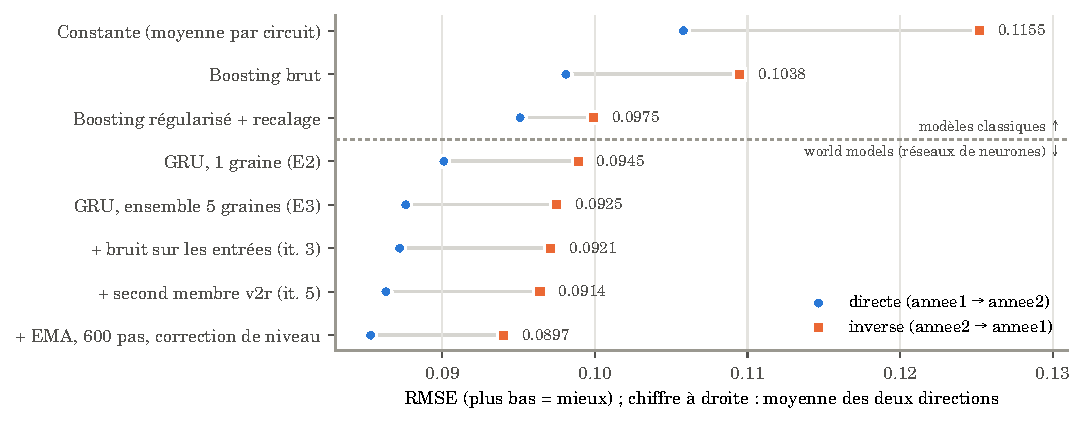
\includegraphics[width=\linewidth]{figures/progression.pdf}
\caption{Progression du score, de la constante au modèle final. Chaque ligne relie la RMSE directe (rond) et la RMSE inverse (carré) d'une même configuration.}
\label{fig:progression}
\end{figure}

%=====================================================================
\section{Solution actuelle}

\subsection{Architecture}

Le modèle répond à la question du sujet : état actuel, actions et contexte donnent l'état suivant. L'état est l'état caché d'un GRU. La figure~\ref{fig:archi} montre les trois parties.

\begin{figure}[!htb]
\centering
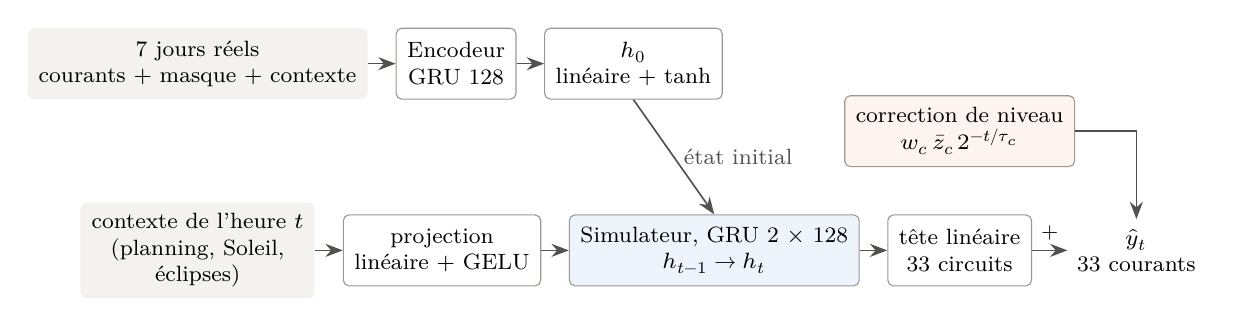
\begin{tikzpicture}[
  font=\footnotesize,
  boite/.style={draw=trait, fill=white, rounded corners=2pt, align=center, minimum height=9mm, inner sep=4pt},
  donnee/.style={draw=none, fill=fond, rounded corners=2pt, align=center, minimum height=9mm, inner sep=4pt},
  fleche/.style={-{Stealth[length=2.2mm]}, draw=encre2, line width=0.6pt},
  node distance=5mm and 3.5mm]
  \node[donnee] (init) {7 jours réels\\courants + masque + contexte};
  \node[boite, right=of init] (enc) {Encodeur\\GRU 128};
  \node[boite, right=of enc] (h0) {$h_0$\\linéaire + tanh};
  \node[donnee, below=13mm of init] (ctx) {contexte de l'heure $t$\\(planning, Soleil,\\éclipses)};
  \node[boite, right=of ctx] (proj) {projection\\linéaire + GELU};
  \node[boite, right=of proj, fill=bleu!8] (sim) {Simulateur, GRU 2 × 128\\$h_{t-1} \to h_t$};
  \node[boite, right=of sim] (tete) {tête linéaire\\33 circuits};
  \node[boite, above=6mm of tete, fill=orange!8] (niv) {correction de niveau\\$w_c\,\bar z_c\,2^{-t/\tau_c}$};
  \node[right=4.5mm of tete, align=center] (y) {$\hat y_t$\\33 courants};
  \draw[fleche] (init) -- (enc);
  \draw[fleche] (enc) -- (h0);
  \draw[fleche] (h0.south) -- node[right, font=\footnotesize, color=encre2] {état initial} (sim.north);
  \draw[fleche] (ctx) -- (proj);
  \draw[fleche] (proj) -- (sim);
  \draw[fleche] (sim) -- (tete);
  \draw[fleche] (tete) -- node[above, font=\footnotesize] {$+$} (y);
  \draw[fleche] (niv.east) -| (y.north);
\end{tikzpicture}
\caption{World model GRU. L'encodeur lit les 7 jours de \code{power\_init} et fixe l'état initial. Le simulateur avance ensuite heure par heure sur le contexte seul, pendant toute la période à prédire.}
\label{fig:archi}
\end{figure}

\paragraph{Encodeur.} Un GRU d'une couche (128 unités) lit les 168 heures de \code{power\_init}. À chaque heure il reçoit le contexte, les 33 courants centrés-réduits et un masque qui indique les mesures présentes. Son dernier état passe par une couche linéaire et une tangente hyperbolique pour donner l'état initial $h_0$ des deux couches du simulateur.

\paragraph{Simulateur.} Un GRU à deux couches de 128 unités (dropout 0.1 entre les couches) avance heure par heure sur le contexte seul, projeté par une couche linéaire suivie d'une GELU. Il ne reçoit jamais ses propres prédictions en entrée. Les courants passés sont résumés dans l'état caché, et une erreur de prédiction ne se réinjecte pas dans l'entrée de l'heure suivante. J'ai fait ce choix à cause de la dérive décrite dans le sujet : une boucle sur les prédictions accumule les erreurs, alors qu'ici le contexte, connu à l'avance, recale le modèle à chaque heure.

\paragraph{Tête et correction de niveau.} Une couche linéaire donne les 33 courants à leur échelle brute ; son biais est initialisé à la moyenne d'entraînement de chaque circuit. On y ajoute une correction tirée de \code{power\_init} :
\[
\hat y_{t,c} = \mathrm{tête}(h_t)_c + w_c \,\bar z_c \, 2^{-t/\tau_c},
\]
où $\bar z_c$ est l'écart moyen centré-réduit du circuit $c$ sur les 7 jours, $w_c$ un poids et $\tau_c$ une demi-vie en heures. $w_c$ et $\tau_c$ sont des paramètres du réseau, appris par descente de gradient avec le reste, initialisés à 0 et 720 heures (30 jours). La forme est la même pour tous les circuits ; seule leur valeur diffère. Avec $w_c = 0$ au départ, le modèle de base est inchangé tant que le gradient ne pousse pas vers la correction.

\subsection{Deux jeux de variables, dix modèles}

Le modèle final fait la moyenne de deux ensembles. Le premier utilise les variables v1 avec du bruit sur les entrées ; le second utilise v2r, sans bruit. Chacun contient cinq modèles entraînés avec des graines différentes. La prédiction est la moyenne des dix modèles, et l'incertitude leur écart-type (variance à l'intérieur de chaque ensemble plus écart entre les deux ensembles). Les deux ensembles se trompent différemment, surtout sur NPWD2551 : leur moyenne passe ce circuit de 0.277 à 0.271 en directe et de 0.236 à 0.228 en inverse.

\begin{table}[!htb]
\centering\small
\caption{Les deux membres de l'ensemble final (poids entraînés sur annee1 + annee2).}
\label{tab:membres}
\begin{tabular}{l r r r r}
\toprule
Membre & Variables construites & Variables gardées & Bruit d'entrée & Paramètres par modèle \\
\midrule
v1  & 65  & 51  & $\sigma = 0.3$ & 336\,995 \\
v2r & 129 & 115 & aucun & 369\,763 \\
\bottomrule
\end{tabular}
\end{table}

\subsection{Entraînement}

Un épisode tire au hasard un point de départ, puis prend 7 jours de démarrage et 365 jours de simulation. Le simulateur s'entraîne donc sur l'horizon réel de l'évaluation. L'épisode est découpé en morceaux de 30 jours : un pas d'optimisation par morceau, et l'état caché passe au morceau suivant sans gradient. La perte est l'erreur quadratique sur l'échelle brute, comme la métrique, avec les heures inconnues masquées. Le tableau~\ref{tab:hyper} donne les réglages.

\begin{table}[!htb]
\centering\small
\caption{Réglages d'entraînement (\code{dio/monde.py}, \code{CONFIG\_DEFAUT}).}
\label{tab:hyper}
\begin{tabularx}{\linewidth}{l X}
\toprule
Réglage & Valeur \\
\midrule
Optimiseur & AdamW, taux maximal $3\cdot10^{-3}$, weight decay $10^{-4}$, plan OneCycle (10 \% de montée) \\
Pas d'optimisation & 600, lots de 32 épisodes, gradient borné à une norme de 1 \\
Moyenne des poids & moyenne exponentielle, décroissance 0.99 ; c'est elle qui est sauvegardée \\
Régularisation & dropout 0.1, bruit gaussien 0.3 sur les entrées normalisées (membre v1) \\
Entrées & variables quasi constantes écartées, bornage à la plage d'entraînement, z-scores bornés à $\pm 5$ \\
Données & annee1 et annee2 fusionnées en une période continue : les épisodes traversent la frontière \\
Durée & 1453 s sur un CPU de 16 cœurs, une graine par processus, en même temps que les ablations ; prédiction 8 s ; poids 6.9 Mo en float16 \\
\bottomrule
\end{tabularx}
\end{table}

La fusion des deux périodes ne concerne que les poids livrés. Elle n'est pas mesurable en validation, où une seule période sert à l'entraînement. Le code utilise CUDA s'il est disponible ; je n'ai pas encore chronométré l'entraînement sur un GPU T4.

\subsection{Dernière session d'améliorations}

La session sur la branche \code{ameliorations} a ajouté trois changements au modèle de l'itération 5 : la moyenne exponentielle des poids, 600 pas au lieu de 300, et la correction de niveau. Les autres pistes n'ont rien apporté (tableau~\ref{tab:session}).

\begin{table}[!htb]
\centering\small
\caption{Session d'améliorations. Les essais B à F sont criblés à 300 pas et comparés à la ligne C1 (ou à la référence pour B1).}
\label{tab:session}
\begin{tabularx}{\linewidth}{l X r r r}
\toprule
 & Changement & Directe & Inverse & Moyenne \\
\midrule
Réf. & ensemble mixte de l'itération 5, relancé sur cette machine & 0.0863 & 0.0964 & 0.0914 \\
A1 & moyenne exponentielle des poids 0.98, 300 pas & 0.0863 & 0.0965 & 0.0914 \\
A2 & moyenne exponentielle 0.99, 600 pas & 0.0855 & 0.0961 & 0.0908 \\
B1 & convolution non causale $\pm 24$ h avant le GRU & 0.0868 & 0.0986 & 0.0927 \\
C1 & correction de niveau, 300 pas & 0.0860 & 0.0941 & 0.0900 \\
\rowcolor{fond} \textbf{C2} & \textbf{correction de niveau + moyenne exponentielle 0.99 + 600 pas (retenu)} & \textbf{0.0853} & \textbf{0.0940} & \textbf{0.0897} \\
D1 & réseau plus petit (96), dropout 0.25, weight decay $10^{-3}$ & 0.0867 & 0.0937 & 0.0902 \\
D2 & bruit 0.3 aussi sur le membre v2r & 0.0860 & 0.0941 & 0.0900 \\
E1 & troisième membre (v2r, taille 64, morceaux de 15 jours) & 0.0861 & 0.0942 & 0.0902 \\
F1 & décalage aléatoire constant par épisode sur les entrées & 0.0860 & 0.0947 & 0.0904 \\
\bottomrule
\end{tabularx}
\end{table}

La moyenne exponentielle seule ne change rien à 300 pas, parce que le plan OneCycle finit déjà avec un taux d'apprentissage presque nul. Avec 600 pas, le gain est de 0.0006 sur les graines 0 à 4 et de 0.0011 sur les graines 5 à 9, et les deux directions s'améliorent à chaque fois. La correction de niveau apporte surtout en inverse ($-0.0024$) ; elle a été confirmée sur les graines 5 à 9 ($-0.0013$), puis à 600 pas.

Les poids appris pour la correction vont surtout à NPWD2531 et NPWD2851, les deux circuits dont le niveau change le plus entre les périodes (tableau~\ref{tab:niveaux}). Dans les poids livrés, les demi-vies apprises vont de 637 à 890 heures selon le circuit (26.5 à 37 jours). La figure~\ref{fig:niveau} montre l'effet sur NPWD2531 en validation inverse : sur les 90 premiers jours, la RMSE de ce circuit passe de 0.527 à 0.447, et de 0.263 à 0.241 sur toute la période. La correction ne rattrape qu'un tiers environ du niveau réel au départ, et s'éteint avant le retour du circuit à 0.6 vers le jour 70.

\begin{figure}[!htb]
\centering
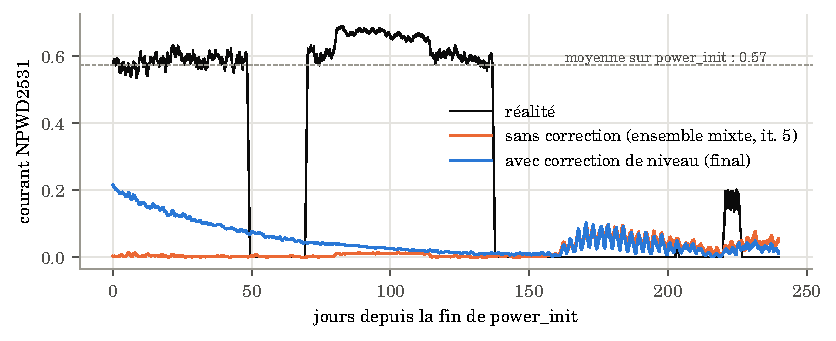
\includegraphics[width=\linewidth]{figures/niveau.pdf}
\caption{NPWD2531 pendant les 240 premiers jours de la validation inverse (moyennes journalières glissantes). Ce circuit vaut 0.57 sur \code{power\_init} mais 0.013 en moyenne sur la période d'entraînement.}
\label{fig:niveau}
\end{figure}

%=====================================================================
\section{Résultats de la solution actuelle}

\subsection{Score global}

Le tableau~\ref{tab:final} compare le modèle final aux deux baselines sur les deux validations. Le gain sur la constante est de 22 \% en moyenne, contre 16 \% pour le boosting.

\begin{table}[!htb]
\centering\small
\caption{RMSE sur les deux validations. Les prédictions ont été regénérées pour ce rapport à partir des poids de \code{runs/c2\_niveau\_600} et retrouvent les scores du journal.}
\label{tab:final}
\begin{tabular}{l r r r r}
\toprule
Modèle & Directe & Inverse & Moyenne & Gain vs constante \\
\midrule
Constante & 0.1058 & 0.1252 & 0.1155 & -- \\
Gradient boosting + recalage & 0.0951 & 0.0999 & 0.0975 & $-15.6$ \% \\
\textbf{World model final} & \textbf{0.0853} & \textbf{0.0940} & \textbf{0.0897} & $\mathbf{-22.3}$ \% \\
\bottomrule
\end{tabular}
\end{table}

\subsection{Dérive sur la période simulée}

La figure~\ref{fig:derive} donne la RMSE de chaque bloc de 30 jours, du début à la fin de la simulation (23 blocs, le dernier ne couvre que 20 jours). Le world model fait mieux que la constante sur 21 blocs sur 23 en directe et sur les 23 en inverse ; il fait mieux que le boosting sur 17 et 18 blocs.

On ne voit pas de dérive qui croît avec le temps, contrairement au premier GRU. En directe, la RMSE vaut 0.064 et 0.060 sur les deux premiers mois et 0.102 sur le dernier ; en inverse, le dernier mois est le meilleur (0.058). L'erreur suit plutôt les phases de la mission : les courbes du modèle et de la constante sont corrélées (0.58 en directe, 0.69 en inverse), donc les mois difficiles sont ceux où les circuits s'éloignent le plus de leur niveau habituel. Les pics du 8\textsuperscript{e} mois en directe (0.122) et du 4\textsuperscript{e} mois en inverse (0.143) touchent les trois modèles.

\begin{figure}[!htb]
\centering
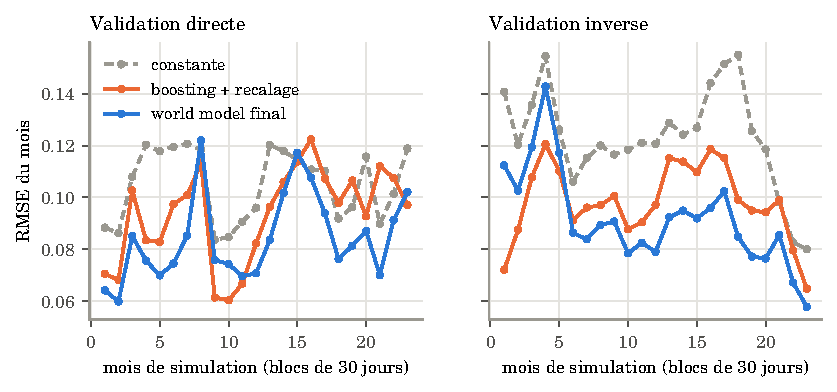
\includegraphics[width=\linewidth]{figures/derive.pdf}
\caption{Courbe de dérive : RMSE par bloc de 30 jours après la fin de \code{power\_init}, pour la constante, le boosting avec recalage et le world model final.}
\label{fig:derive}
\end{figure}

\subsection{Rêve contre réalité}

La figure~\ref{fig:reve} compare la simulation et la réalité sur toute la validation directe, avec la bande de $\pm 2$ écarts-types de l'ensemble. Le modèle suit bien la consommation totale et les variations lentes de NPWD2532. Sur NPWD2551, il retrouve les périodes hautes d'octobre à décembre 2010 et de juillet à novembre 2011, mais pas les coupures brusques, comme les cinq semaines à zéro entre fin janvier et fin février 2011.

\begin{figure}[!htb]
\centering
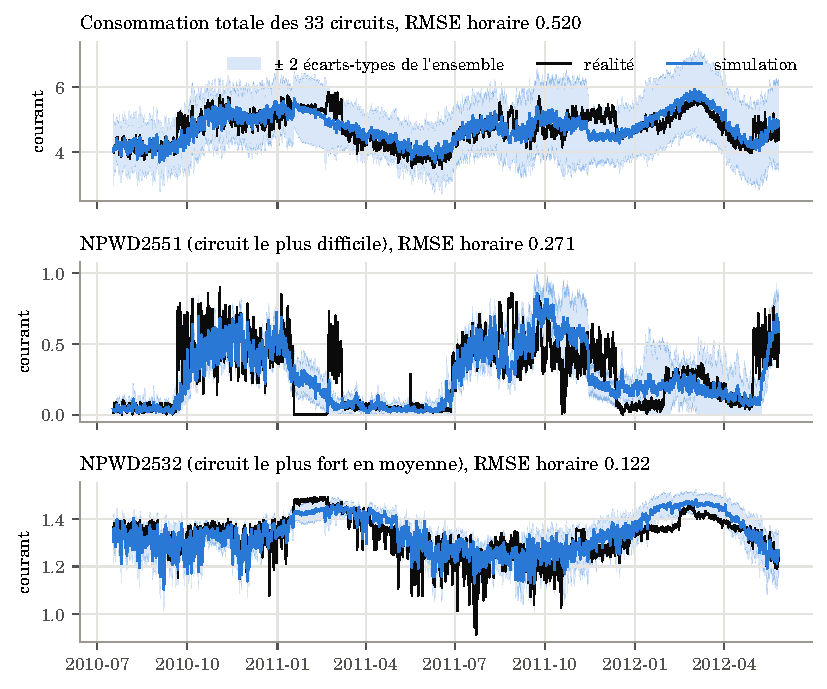
\includegraphics[width=\linewidth]{figures/reve.pdf}
\caption{Rêve contre réalité sur la validation directe (entraînement sur annee1 seul, simulation de annee2 à partir de ses 7 premiers jours). Moyennes glissantes sur 24 h pour la lisibilité ; les RMSE sont horaires. Pour le total, la bande additionne les écarts-types des circuits, ce qui majore l'incertitude.}
\label{fig:reve}
\end{figure}

\subsection{Erreurs par circuit}

Deux circuits font plus de la moitié de l'erreur : NPWD2551 (31 \% de l'erreur quadratique totale en directe) et NPWD2451 (21 \%). Ce sont les plus variables, avec des changements de régime rapides. La figure~\ref{fig:circuits} compare, pour les dix circuits qui pèsent le plus, le modèle final à deux constantes : celle apprise sur annee1, et celle qui vaudrait exactement la moyenne réelle d'annee2. La seconde est inaccessible en pratique ; elle indique l'erreur qui reste quand seul le niveau est juste.

\begin{figure}[!htb]
\centering
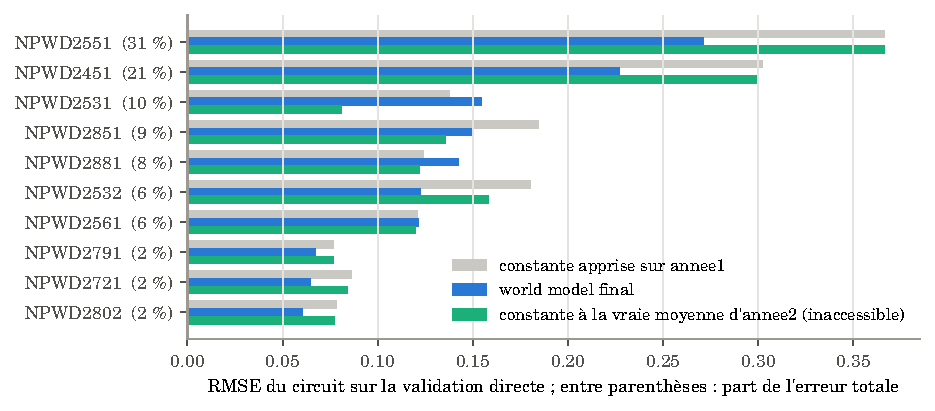
\includegraphics[width=\linewidth]{figures/circuits.pdf}
\caption{RMSE par circuit en validation directe, pour les dix circuits qui contribuent le plus à l'erreur.}
\label{fig:circuits}
\end{figure}

Sur NPWD2551, NPWD2451, NPWD2532 et NPWD2851, le modèle bat nettement les deux constantes : il prédit les variations, pas seulement le niveau. Trois circuits restent mal traités. NPWD2531 (0.154) et NPWD2881 (0.143) sont prédits plus mal que la constante apprise sur annee1 (0.138 et 0.124), et NPWD2561 ne fait pas mieux qu'elle. Pour NPWD2531, l'écart à la constante idéale (0.081) vient du changement de niveau entre les périodes, que ni le contexte ni la correction de niveau ne suffisent à expliquer.

\subsection{Incertitude}

L'écart-type de l'ensemble sert de mesure d'incertitude. Sur la validation directe, 77.3 \% des valeurs réelles tombent dans la bande $\pm 2$ écarts-types, et 79.3 \% en inverse. Une incertitude bien calibrée de forme gaussienne donnerait environ 95 \%. L'ensemble sous-estime donc son incertitude : les dix modèles se trompent souvent dans le même sens, surtout lors des changements de niveau qu'aucun d'eux n'a vus à l'entraînement. La bande reste utile pour repérer les périodes où les modèles divergent, mais elle ne doit pas être lue comme un intervalle à 95 \%.

\subsection{Ablations}

Chaque ablation retire un groupe d'entrées ou la mémoire, et réentraîne le membre v1 (configuration finale, 2 graines par direction). « Sans mémoire » remplace l'encodeur et le GRU par un réseau sans état ; la correction de niveau, qui lit \code{power\_init}, disparaît avec.

\begin{table}[!htb]
\centering\small
\caption{Ablations (\code{outils/ablations.py}, détail dans \code{docs/ABLATIONS.md}).}
\label{tab:ablations}
\begin{tabular}{l r r r}
\toprule
Variante & Directe & Inverse & Écart moyen vs complet \\
\midrule
complet & 0.0864 & 0.0941 & -- \\
sans éclipses & 0.0879 & 0.0957 & $+0.0016$ \\
sans \code{saaf} (Soleil) & 0.0870 & 0.0989 & $+0.0027$ \\
sans \code{dmop} (commandes) & 0.0885 & 0.0958 & $+0.0019$ \\
sans mémoire & 0.0891 & 0.1055 & $+0.0071$ \\
\bottomrule
\end{tabular}
\end{table}

\begin{figure}[!htb]
\centering
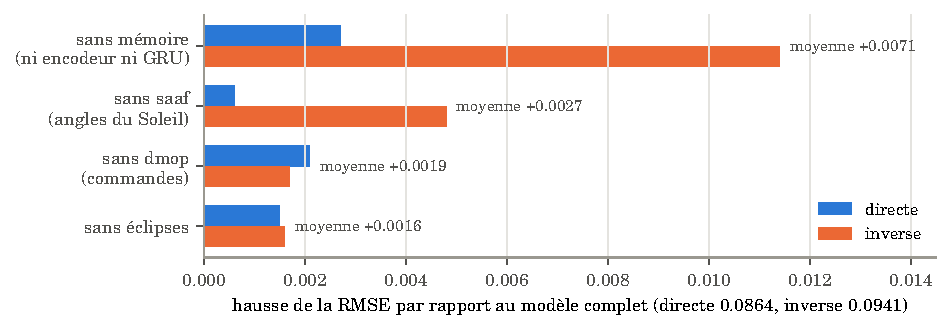
\includegraphics[width=\linewidth]{figures/ablations.pdf}
\caption{Hausse de la RMSE quand on retire un élément du modèle, par direction.}
\label{fig:ablations}
\end{figure}

La mémoire est l'élément qui compte le plus, surtout en inverse ($+0.0114$) : sans encodeur, le modèle ne sait pas dans quel état se trouve le satellite au début de la période. Les angles solaires comptent surtout en inverse ($+0.0048$ contre $+0.0006$ en directe). Les commandes \code{dmop} et les éclipses ont un effet plus faible mais présent dans les deux directions. Avec la configuration actuelle, les commandes pèsent plus qu'avec le modèle de l'étape E3 ($+0.0019$ contre $+0.0009$), et la mémoire aussi ($+0.0071$ contre $+0.0049$). Ces écarts portent sur deux graines ; pour les éclipses, \code{dmop} et \code{saaf}, ils restent proches du bruit de graine mesuré (0.0015).

%=====================================================================
\section{Limites et travail restant}

\begin{itemize}
  \item Le bonus pilote n'est pas commencé. Le modèle peut déjà servir de simulateur : modifier le planning (\code{dmop}, \code{ftl}) en gardant les mêmes fenêtres de communication, puis comparer la consommation simulée. Il faudra limiter les changements à des plannings proches de ceux vus à l'entraînement, car le modèle borne ses entrées à cette plage.
  \item NPWD2531 et NPWD2881 restent moins bien prédits qu'une constante. La correction de niveau ne rattrape qu'une partie de l'écart initial et s'éteint en un mois environ.
  \item L'incertitude est sous-estimée : la couverture de la bande $\pm 2\sigma$ est de 77 à 79 \%. Un facteur d'échelle appris sur la validation corrigerait la largeur de la bande sans toucher à la prédiction.
  \item La référence de l'itération 5 a été reproduite à l'identique sur une seconde machine. La durée sur GPU T4 n'est pas mesurée ; sur CPU 16 cœurs, l'entraînement complet prend 1453 s.
  \item L'entraînement final sur annee1 et annee2 fusionnées n'a pas pu être validé, faute de période de validation indépendante.
\end{itemize}

%=====================================================================
\appendix
\section{Reproduire les résultats}

Environnement : Python 3.13, \code{uv sync} (ou \code{pip install -r requirements.txt}).

\begin{small}
\begin{verbatim}
python train.py                                   # modèle final -> poids/
python predict.py --test_dir DOSSIER --out predictions.csv
python outils/valider.py --nom essai --modele gru_mixte   # directe + inverse
python outils/ablations.py
python outils/demo.py --poids runs/c2_niveau_600/directe
python docs/rapport/figures.py --preds DOSSIER_PREDICTIONS   # figures de ce rapport
\end{verbatim}
\end{small}

Le journal complet des essais, avec les durées, est dans \code{docs/RESULTATS.md}.

\end{document}
